\documentclass[11pt]{article}
\usepackage[utf8]{inputenc}
\usepackage[parfill]{parskip}  % no indents
\usepackage{geometry}
 \geometry{
 a4paper,
 left=25mm,
 top=40mm,
 right=25mm,
 bottom=27mm
 }
\usepackage{natbib}  % references
\usepackage{graphicx}  % plots
\usepackage{scrextend}  % indent authors
\usepackage{amsmath}  % math typesetting
\usepackage{graphicx}
\usepackage{subcaption}

% typeset in sans serif to match the prompt
\usepackage{lmodern}
\renewcommand{\familydefault}{\sfdefault}
% correct the section heading size
\usepackage{titlesec}
\titleformat*{\section}{\normalsize\bfseries}

%%%%%%%%%%%%%%%%%%%%%%%%%%%%%%%%%%%%%%%%%%%%%%%
\begin{document}
\raggedright  % don't stretch to right edge

% =============================================
\vspace*{80pt}
{\LARGE \textbf{Global sensitivity analysis of model parameters in aeroelastic wind-turbine codes}}
\vspace*{28pt}

\begin{addmargin}[2.5cm]{0em}% 1em left, 2em right
\textbf{P. Kumar$^{\boldsymbol{\mathsf{1}}}$, B. Sanderse$^{\boldsymbol{\mathsf{1}}}$}

$^{\mathsf{1}}$ Centrum Wiskunde \& Informatica, Science Park 123, Amsterdam.

%$^{\mathsf{2}}$Address 2.
%\vspace{12pt}

Author contact email: b.sanderse@cwi.nl

Keywords: aero-elastic turbine model, BEM, sensitivity analysis, model uncertainty
\end{addmargin}

% =============================================
\section{Introduction}
Aeroelastic models such as the Blade Element Momentum (BEM) method \cite{HandBook} continue to play a critical role in the design, development and optimization of modern wind turbines. The accuracy of BEM predictions is affected to by uncertainties and inaccuracies, for example in the external conditions (wind parameters), in the turbine specification (geometric parameters), and in the BEM equations itself (model parameters). For the purpose of design, uncertainty quantification and optimization, is it crucial to limit the number of parameters, typically by performing sensitivity studies. Most studies focused on the effect of uncertainties in the external conditions and in the geometry, see e.g.\ \cite{Echeverria2017,Matthaus2017,Murcia2018,Robertson2018}.

\section{Objectives}
The long-term objective of this study is to develop calibrated BEM models that give users an indication of the uncertainty associated with the predictions (loads, power, etc.) originating not only from external conditions and geometry, but also from the model formulation itself. For this purpose, we will calibrate the model parameters present in BEM models. Examples of such model parameters are the time constant in dynamic stall models, the wake correction factor, the tip loss model parameter, and the lift- and drag-polars \cite{Sayed2019}. In order to limit the number of model parameters involved in the calibration process, \textit{the objective of the current study is to perform a global sensitivity study of the outputs of the BEM model towards both geometric and model uncertainties}.

%In the past a number of sensitivity studies have been performed to understand the influence of input parameters on different turbine response, e.g.\ \cite{moriarty2002effect, eggers2003wind, McKay2014, dykes2014sensitivity, Robertson2018}. Many studies have confirmed that the wind parameters especially the wind speed and wind speed standard deviation have the most influence on aerodynamical performance of turbines. For example, in the of an upstream turbine, the wind speed is most sensitive to power production. Furthermore, wind speed in combination with wind speed standard deviation has a large influence on the power production of turbines operating in the wake of an upstream turbine. Among operational factors, the rotor RPM is the most sensitive to power production. [More on parameter sensitivities on structural loads]

% In particular, BEM models are employed to predict turbine response such as the structural loads and power outputs.

%`These tools use simplified methods such as BEM to find the unsteady aerodynamic loads and 1D structural models to determine the deformations. They are computationally cheap, but they are based on different corrections to account for the unsteadiness and the 3D effects.' \cite{Sayed2019}

%[Sensitivity on the polars as novel element]

%[Mention this study is a part of IEA Task29 project and WindTrue.

%In this work, we also study the effect of manufacturing tolerances on the turbine response. Usually, there are some discrepancy between the  manufactured and nominally prescribed design of the turbine blade leading to a suboptimal performance. For BEM models, the turbine shape is described as a series of airfoils along the span of the blade where each airfoil shape is computed using the three quantities: chord length, thickness and twist. We perturb these three quantities to obtain a perturbed turbine blade and analyze with sections that have more influence on output quantities. 



% =============================================

% =============================================
\section{Methodology}
To compute parameter sensitivities we use a global sensitivity analysis based on the Sobol expansion approach, which decomposes the total variance of the quantity of interest (model output) into contributions from individual parameters and their combinations, similar to \cite{Echeverria2017,Murcia2018,Rinker2016}. We employ the uncertainty quantification toolbox \texttt{UQLab} \cite{uqlab}, which computes the Sobol indices from a sparse polynomial chaos expansion. \texttt{UQLab}'s modular structure allows for easy integration with available BEM codes. 

The geometric uncertainties currently considered are chord and twist distribution, whereas the model uncertainty enters via uncertainty in lift- and drag-polars. In order to express the chord, twist, lift and drag distributions along the turbine blade, an efficient parameterization is needed that gives flexible control over the prescribed uncertainty while limit the number of required parameters. We have chosen to use Non-Uniform Rational Basis Splines (NURBS) for this purpose, similar to \cite{Echeverria2017}. 

% =============================================
\section{Results}
The aeroelastic code that we use is the \texttt{ECN Aero-Module} \cite{Boorsma2012} and the turbine is the 2MW NM80 turbine from the DANAERO project \cite{Troldborg2013} with a blade radius of 38.8m. The data for lift ($Cl$) and drag ($Cd$) polars are available at four locations along the blade radius at 11.87m, 17.82m, 28.97m and 35.53m. The reference value of polars are obtained from wind-tunnel experiment with 3D corrections. Random samples of chord, twist, lift- and drag-polars are obtained by perturbing the control points with a uniformly distributed random variable. For chord and twist, we independently perturb control points at different locations as shown in Fig. \ref{fig:samples} (a) - (b). For $Cl$ and $Cd$, all control points are perturbed using a same random number.

In Fig. \ref{fig:Sobol}, we show the total order Sobol indices as a measure of sensitivity for different geometric and model parameters on power production. The control points are named

\begin{figure}[h!]
  \centering
  \begin{subfigure}[b]{0.4\linewidth}
    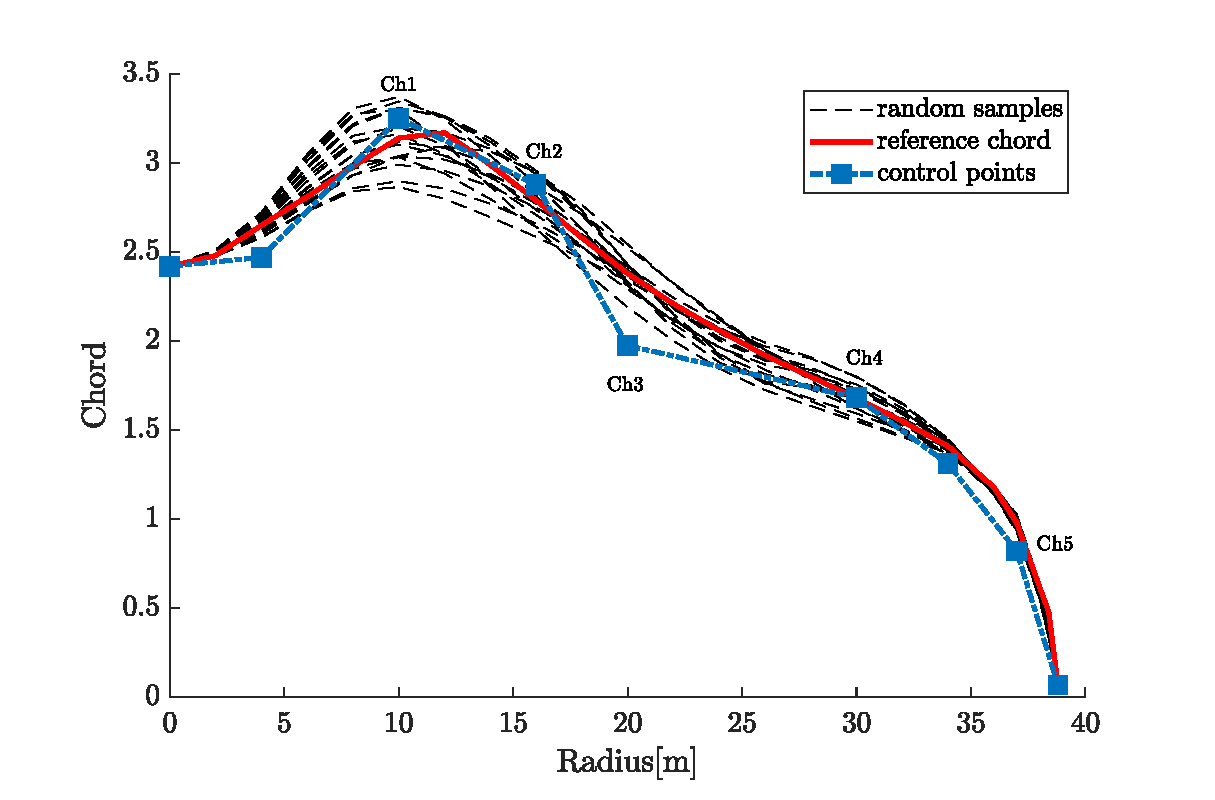
\includegraphics[width=\linewidth]{Chord_samples_torque.eps}
   % \caption{Coffee.}
  \end{subfigure}
  \begin{subfigure}[b]{0.4\linewidth}
    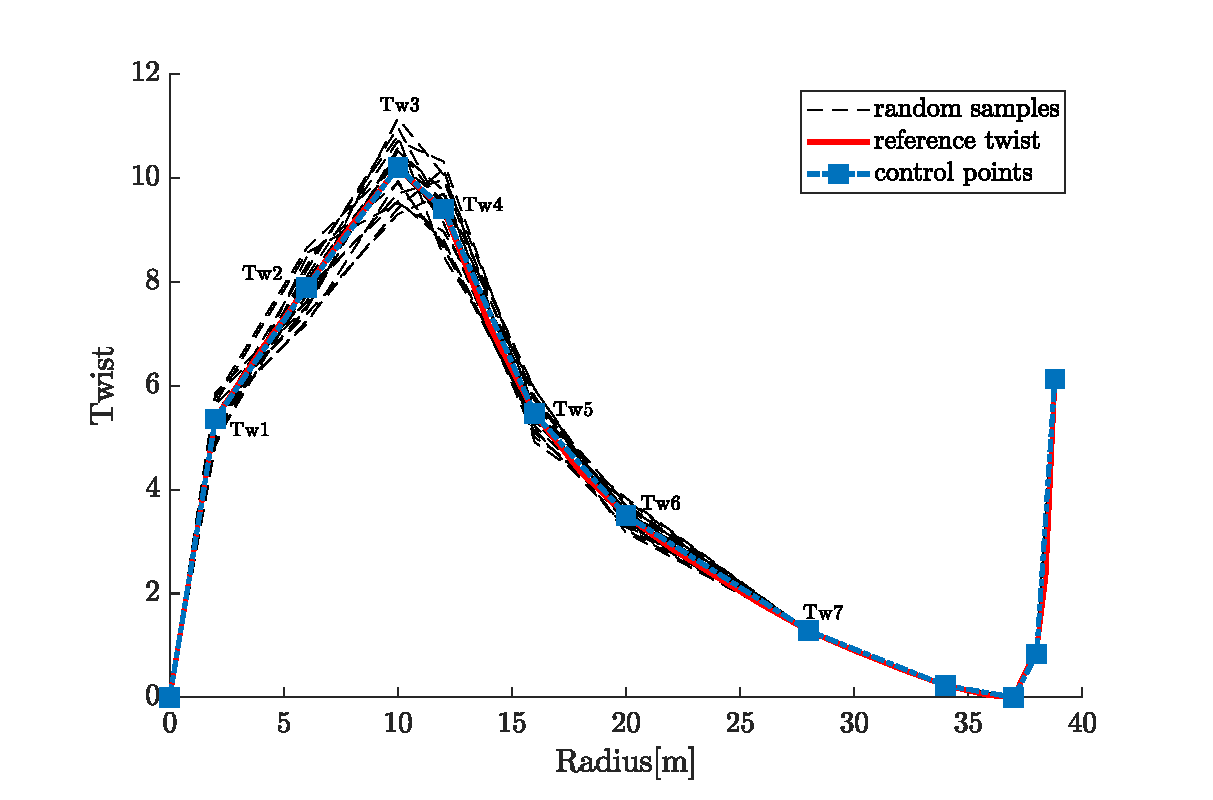
\includegraphics[width=\linewidth]{Twist_samples_torque.eps}
   % \caption{More coffee.}
  \end{subfigure}
  
  \begin{subfigure}[b]{0.4\linewidth}
    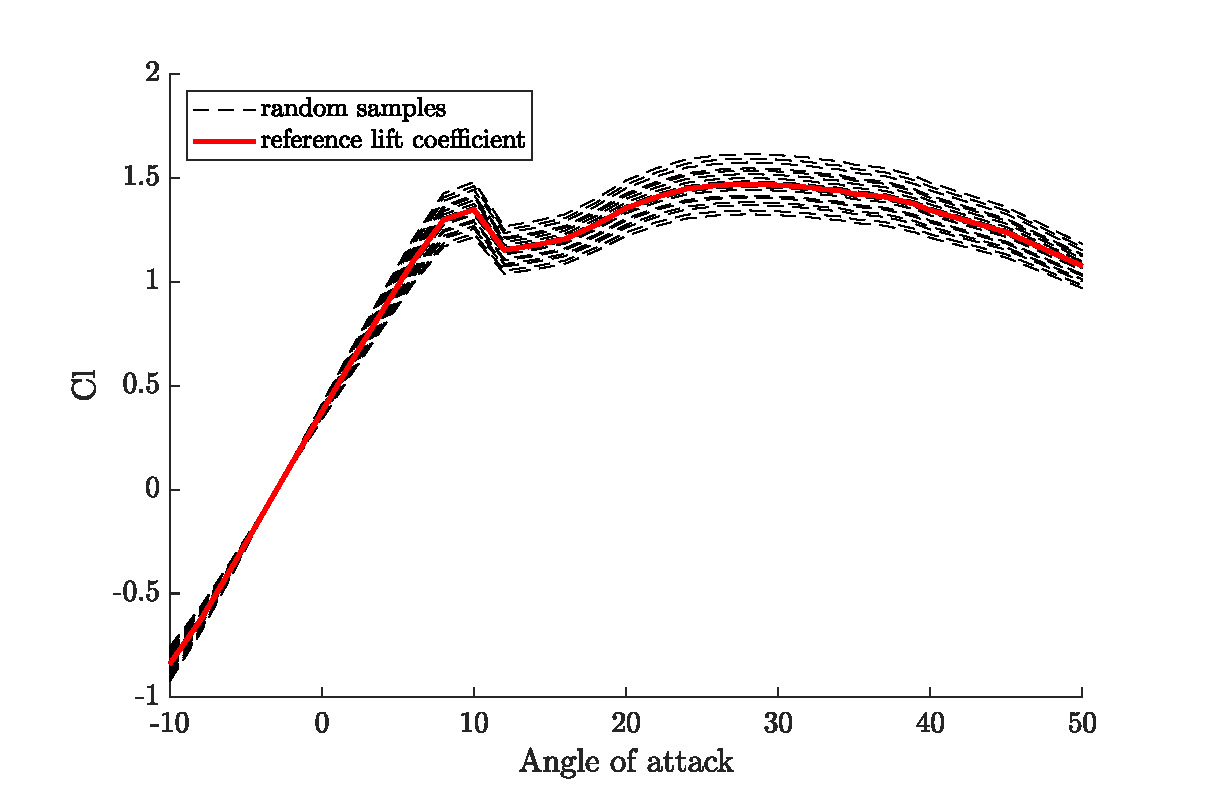
\includegraphics[width=\linewidth]{Cl_samples_torque.eps}
    %\caption{Coffee.}
  \end{subfigure}
  \begin{subfigure}[b]{0.4\linewidth}
    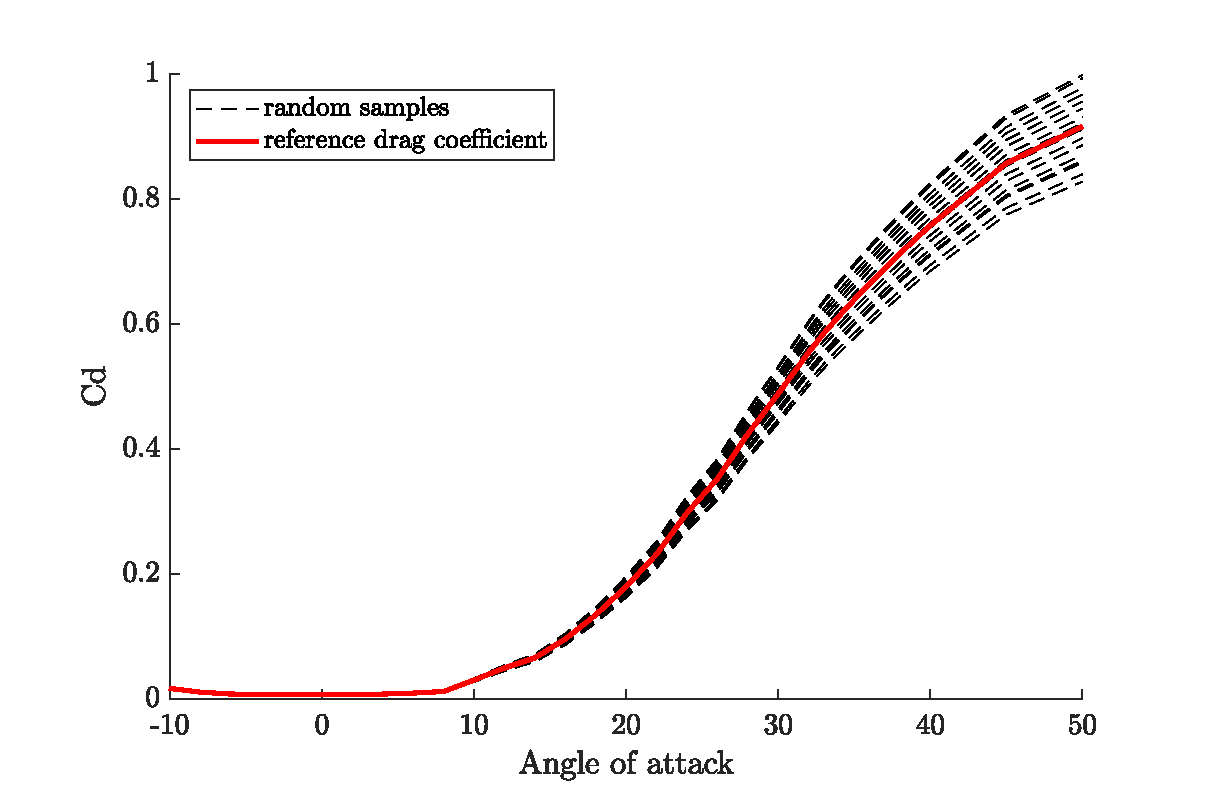
\includegraphics[width=\linewidth]{Cd_samples_torque}
    %\caption{More coffee.}
  \end{subfigure}
  \caption{Random realization of twist, chord, lift- and drag-polars.}
  \label{fig:samples}
\end{figure}
\begin{figure}[h!]
  \centering
    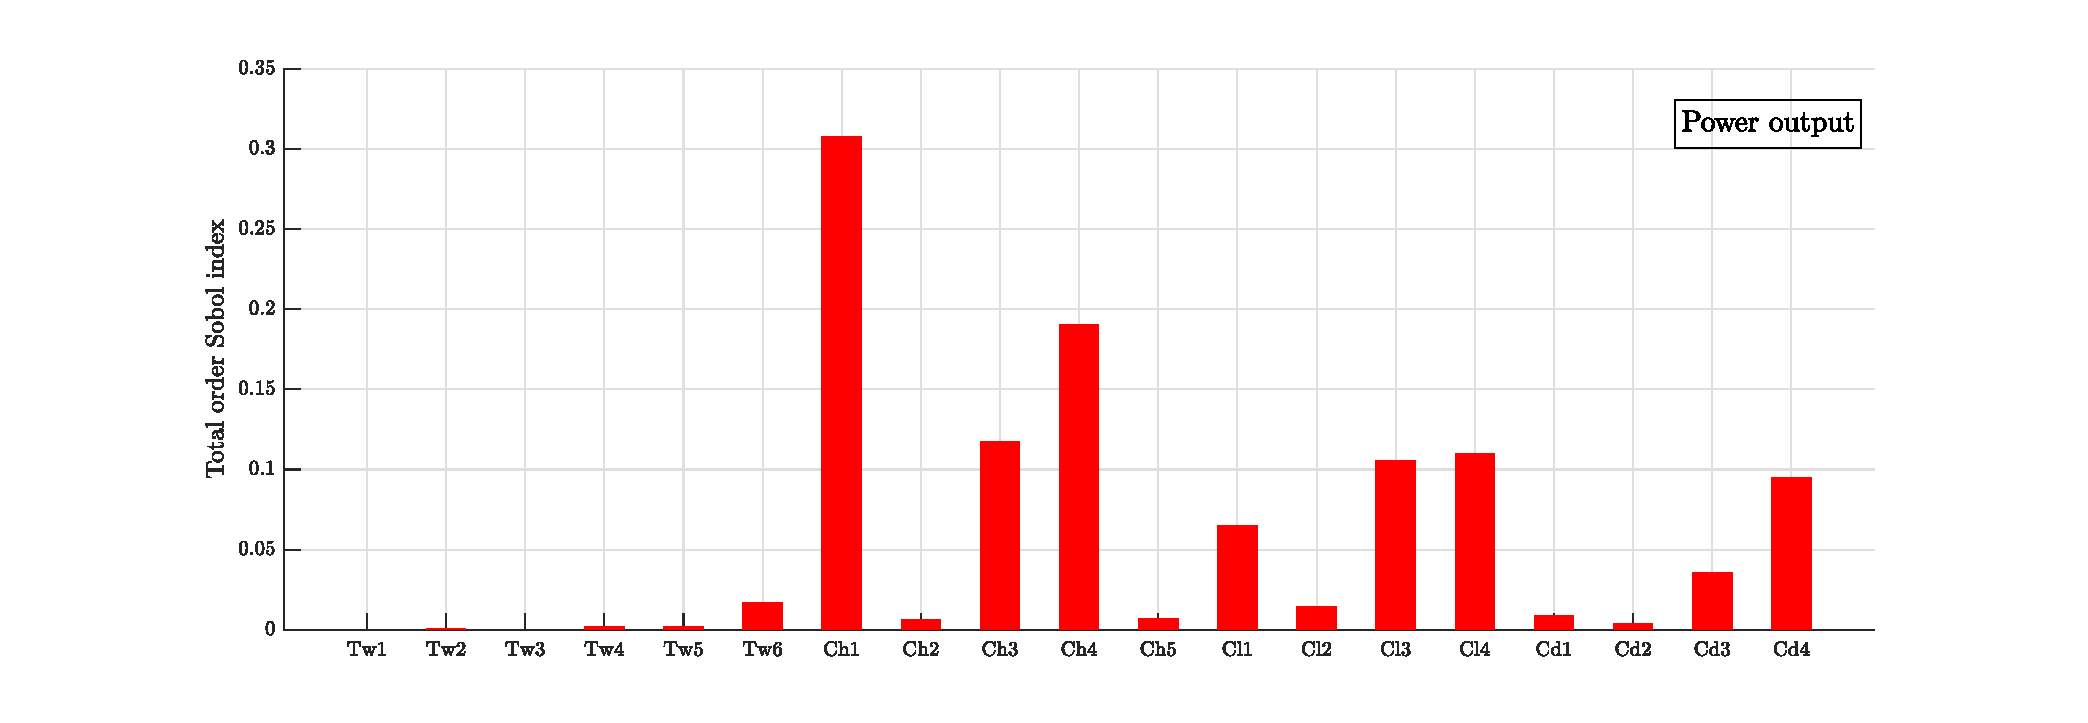
\includegraphics[width=\linewidth]{SA_Power_Chord_Twist_CD_CL_torque.eps}
  \caption{Total order Sobol indices for the sensitivity analysis of geometrical and model parameters.}
   \label{fig:Sobol}
\end{figure}
% =============================================
\section{Conclusions}
Global sensitivity analysis is a powerful tool to identify important input parameters associated with aeroelastic models. Sobol indices computed using sparse polynomial expansion is very efficient and can be used to analyze large number of input parameters. In the full paper, we will present a sensitivity assessment with a more model parameters.
% =============================================
\bibliographystyle{abbrv}
\bibliography{../references,../Mendeley_refs}

\end{document}
